\title{Qt Installation}
\author{John Till}
\date{}

\documentclass[12pt]{article}

\usepackage[a4paper, margin=0.75in]{geometry}
\usepackage[colorlinks=true,urlcolor=blue]{hyperref}
\usepackage{graphicx}

\begin{document}

\makeatletter
\renewcommand{\@maketitle}{
\newpage
\null
\vskip 2em
\begin{center}
{\LARGE \@title \par}
\end{center}
\par
} \makeatother

\maketitle

The Qt installer can be downloaded from \href{https://www.qt.io/download}{https://www.qt.io/download}. The open-source version is free subject to a more restrictive licensing agreement which you can learn about on the Qt website. The installer may take a while to retrieve the information it needs before you can choose the installation options.

Once inside the installer, you should expand the latest version of Qt. This will include an option of which compilers you want Qt to be compatible with. If you have Visual Studio installed, you can select an appropriate MSVC option. If you have MinGW or no compiler installed, you can select one of the MinGW options. You should also select ``Qt Charts'' since the code examples rely on this library.

\begin{figure}[h]
	\centering
		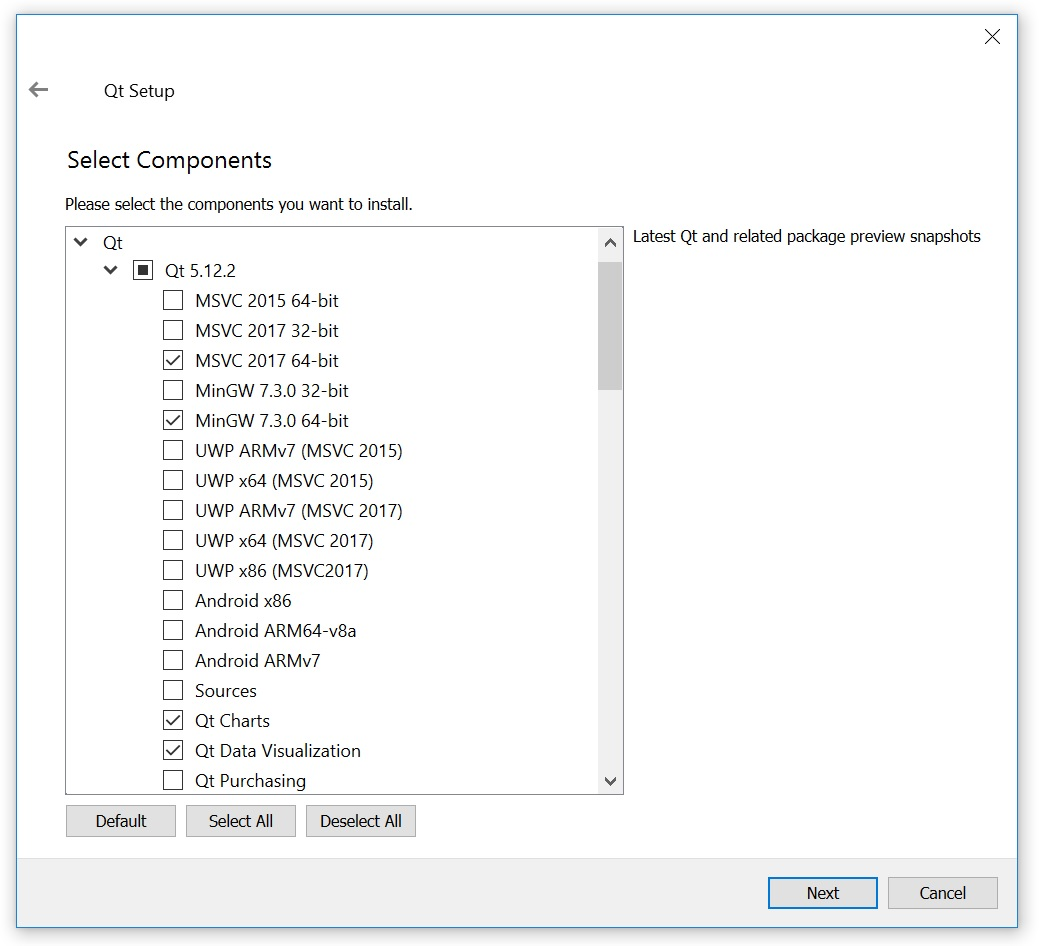
\includegraphics[width=1.00\textwidth]{fig/installer.jpg}
\end{figure}
\clearpage

If you selected a MinGW option not present on your computer, you should also install the compiler itself under the ``Developer and Designer Tools'' section:

\begin{figure}[h]
	\centering
		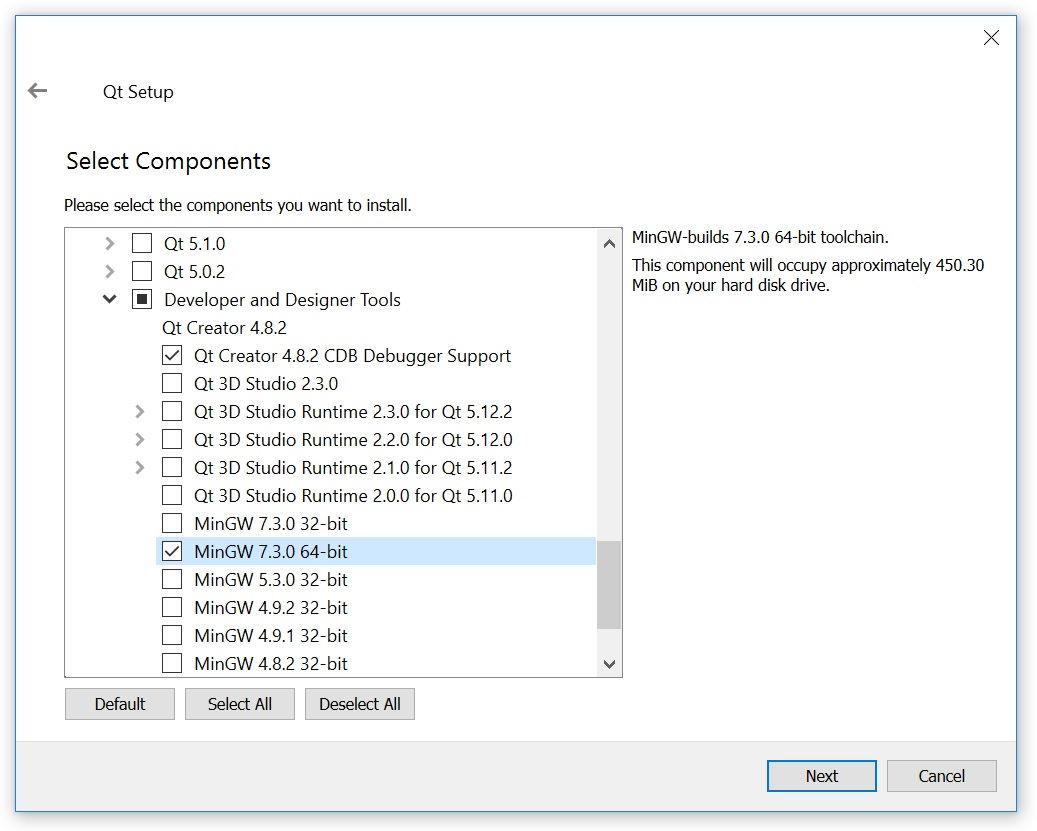
\includegraphics[width=1.00\textwidth]{fig/installer_mingw.jpg}
\end{figure}
\clearpage

The installer will take a while to setup Qt. Once it is finished, you can open up a .pro file to work with a Qt project. Qt will prompt you to choose which compiler to associate with the project, and the script should work regardless of your choice.

\begin{figure}[h]
	\centering
		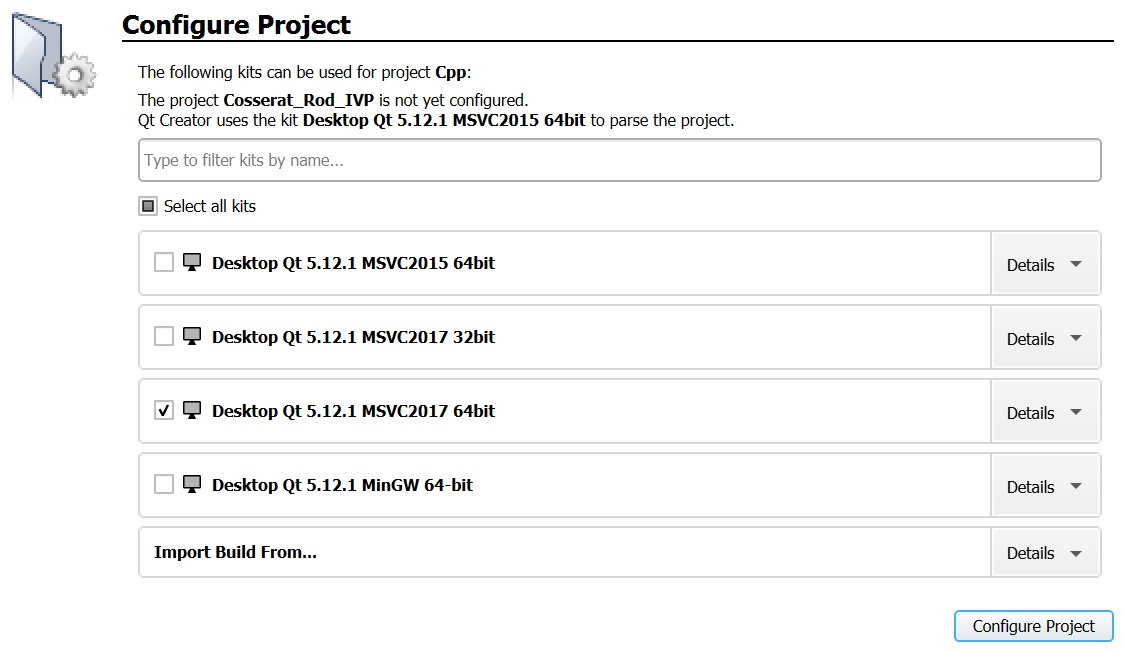
\includegraphics[width=0.85\textwidth]{fig/configuration.jpg}
\end{figure}

Once a project is configured, you can compile and run it with the button shown below:

\begin{figure}[h]
	\centering
		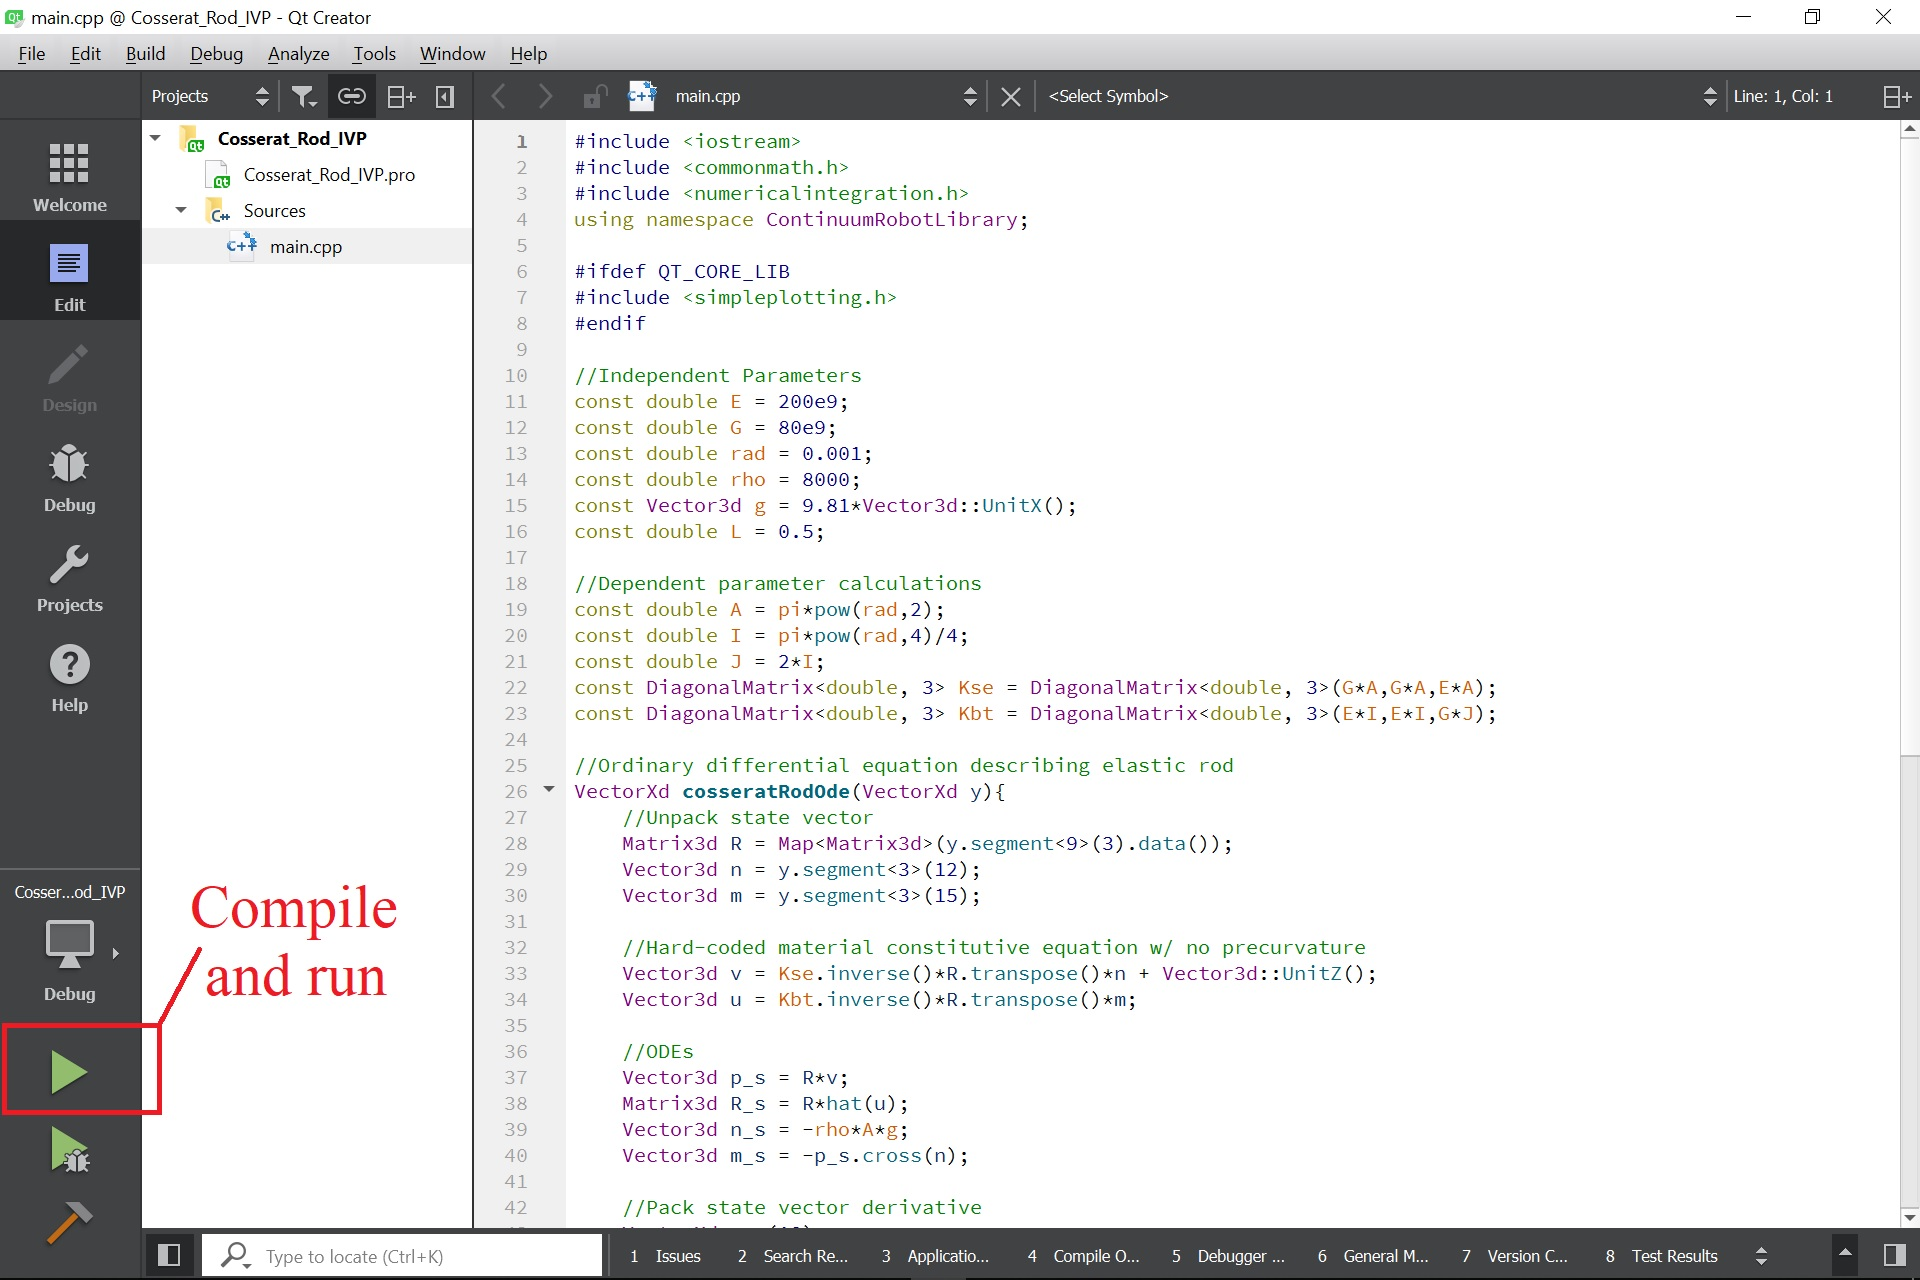
\includegraphics[width=0.9\textwidth]{fig/compile_and_run.jpg}
\end{figure}
\clearpage

In addition to compiling, Qt has an extra step ``qmake'' which needs to be run when the .pro file is modified (which includes adding or removing files from the project) or when Qt functionality is changed within the code, e.g. adding a Qt signal or slot to a class.

\begin{figure}[h]
	\centering
		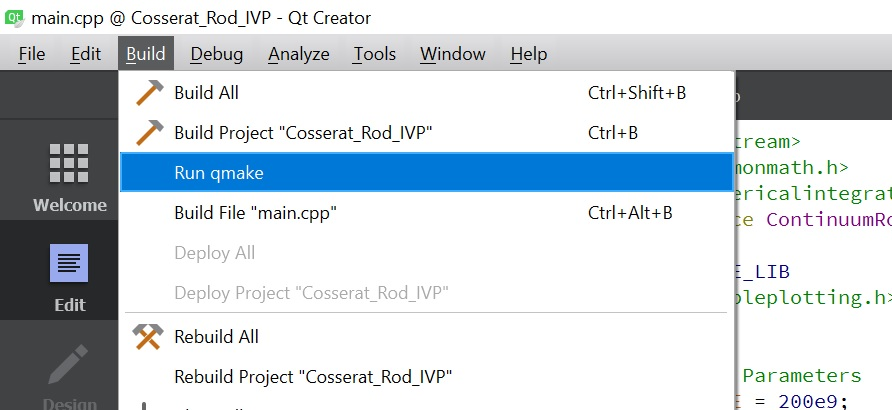
\includegraphics[width=0.9\textwidth]{fig/qmake.jpg}
\end{figure}

Minor changes to code files won't require running qmake again, but it's important to realize it may be necessary.

\end{document}